
\section{Supplementary Figures}

% \begin{figure*}[t]
%   \begin{center}
%   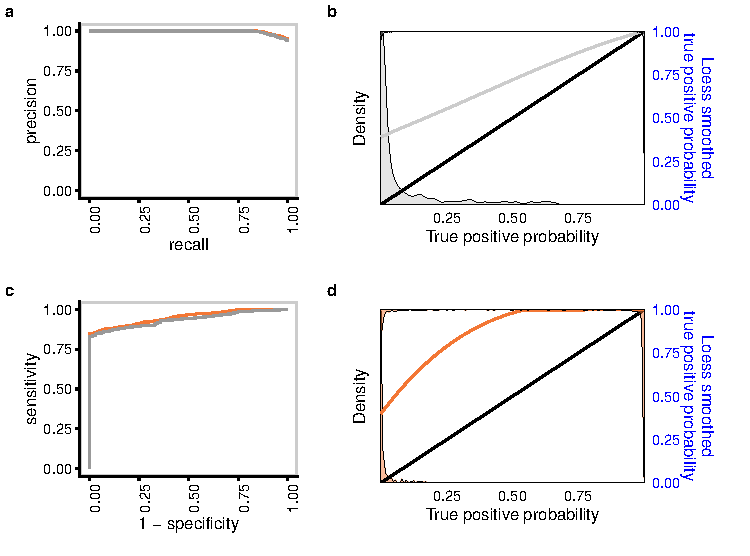
\includegraphics{figures/aml_plot.pdf}
%   \end{center}
%   \caption{Model performance on 300X Whole leukemia genome.
%   \textbf{(a)} Precision/recall curves and \textbf{(c)} Reciever operating characteristic curves.
%   Distribution of estimated true positive probabilities for true positive (top) and true negative (bottom) variants for \textbf{b)} the MuTect model and \textbf{d)} the Calibrated model.
%   A perfectly calibrated model would generate the diagonal line.}
%   \label{NAR-aml}
% \end{figure*}

\begin{figure*}
  \begin{center}
  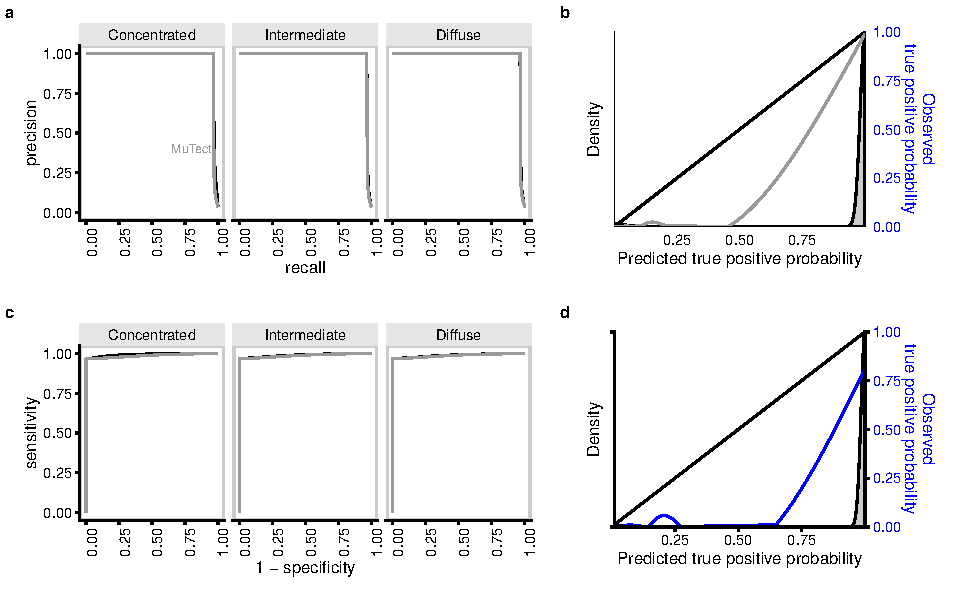
\includegraphics{figures/fig_wgs.pdf}
  \end{center}
  \caption{Model performance on 100X simulated whole genome.
  \textbf{(a)} Precision recall curves and \textbf{(c)} Reciever operating characteristic curves for 3 mutation signatures.
  Distribution of estimated true positive probabilities for true positive (top) and true negative (bottom) variants for \textbf{b)} the MuTect model and \textbf{d)} the BATCAVE model.
  A perfectly calibrated model would generate the diagonal line.}
\label{NAR-wgs_fig}
\end{figure*}

\begin{figure}
  \begin{center}
  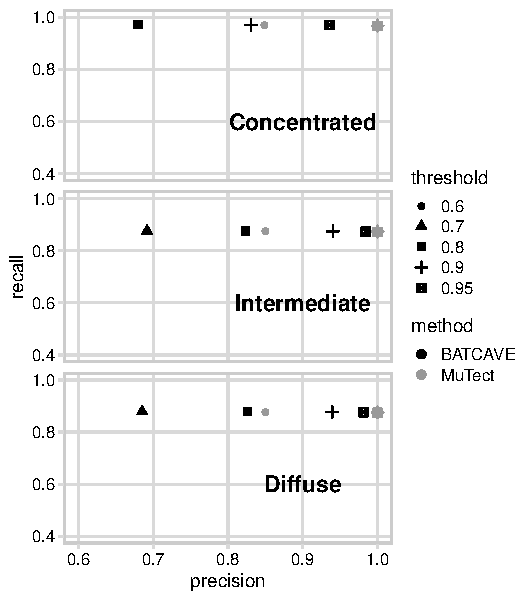
\includegraphics{figures/ppv_wgs.pdf}
  \end{center}
  \caption{Model performance on 500X simulated whole exome. 
  Positive predictive values vs. Recall for three different probability cutoffs. 
  Note the restricted axes to improve readability of points.}
\label{NAR-ppv_wgs_fig}
\end{figure}

\section{Supplememtary Table}

\begin{table*}[b]
  \tableparts{%
  \caption{This is a table with $\mu$, auroc, auprc, ICI, and maybe fraction called?}
  \label{table:01}%
  }{%
  \begin{tabular*}{\textwidth}{@{}lllllllll@{}}
  \toprule
  Depth & Mutation profile & $\mu$ & AUROC & & AUPRC & & ICI & 
  \\
  & & (estimated) & MuTect & BATCAVE & MuTect & BATCAVE & MuTect & BATCAVE
  \\
  \colrule
  100X whole genome & Concentrated & 3.6e-7 & .987 & .993 & .972 & .975 & -- & --
  \\
  100X whole genome & Intermediate & 3.2e-7 & .987 & .989 & .972 & .973 & -- & --
  \\
  100X whole genome & Diffuse & 3.2e-7 & .988 & .989 & .971 & .973 & -- & --
  \\
  500X whole exome & Concentrated & 3.6e-7 & .848 & .929 & .674 & .758 & .138 & .109
  \\
  500X whole exome & Intermediate & 3.6e-7 & .847 & .881 & .677 & .706 & .108 & .112 
  \\
  500X whole exome & Diffuse & 3.6e-7 & .850 & .873 & .676 & .698 & .105 & .116
  \\
  Williams & Actual & 3.6e-8 & -- & -- & .995 & .996 & -- & --
  \\
  Shi & Actual & 3.6e-8 & -- & -- & .972 & .972 & -- & --
  \\
  \botrule
  \end{tabular*}%
  }
  {$\mu$ = per-base mutation rate, AUROC/AUPRC = area under ROC/PRC curve, ICI = Integrated calibration index.}
  \end{table*}


